% !TeX spellcheck = nl_NL
\chapter{Integratie SLAM in het platform}
In dit hoofdstuk wordt het gekozen SLAM algoritme ge\"integreerd in het huidige platform. Er moeten eerst een aantal aanpassingen gemaakt worden aan de architectuur, zowel op vlak van hardware als op vlak van software. Eens de architectuur af is, wordt de prestatie van het SLAM algoritme ge\"evalueerd. Dit gebeurt eerst zonder odometrie van de quadcopter te gebruiken, om erna te zien wat het effect is als er wel odometrie gebruikt wordt. In dit hoofdstuk moet in het achterhoofd gehouden worden dat het uiteindelijke doel erin bestaat dat de quadcopter autonoom een omgeving kan verkennen. Er moet dus ook nagegaan worden of dit mogelijk is met het gebruikte platform.

\section{Aanpassingen architectuur}

\subsection{Aanpassingen hardware}
Om aan SLAM te doen, wordt in dit werk een URG-04LX-UG01 laserscanner van Hokuyo gebruikt. Deze laserscanner haalt een maximale scanfrequentie van \SI{10}{\Hz}. Deze scanner kan gewoon via USB aangesloten worden. Dit levert echter een probleem op, want de RPi\,1 heeft slechts 2 USB-poorten en die zijn reeds in gebruik door de WiFi-dongle en de camera. Omdat het niet mogelijk is nog een USB-HUB toe te voegen aan het platform wegens plaatsgebrek, moet een andere optie gezocht worden. De beste oplossing lijkt ons over te gaan naar de nieuwe RPi\,2. Deze is een stuk krachtiger, en beschikt over 4 USB-poorten, zie tabel \ref{table:RP1vsRPI2}.

\npar Van de gebruikte laserscanner is geweten dat hij vrij veel stroom eist. Dit blijkt dan ook meteen een probleem op te leveren. De RPi2 kan niet voldoende stroom  leveren om zowel de laserscanner als de camera voldoende te voeden. De RPi2 wordt gevoed door de APM. Als de laserscanner ook rechtstreeks gevoed wordt door de APM lijkt dit probleem reeds opgelost. Een foto van de finale versie van het platform is weergegeven in figuur \ref{fig:quadfinal}.

\begin{figure}[h]
	\centering
	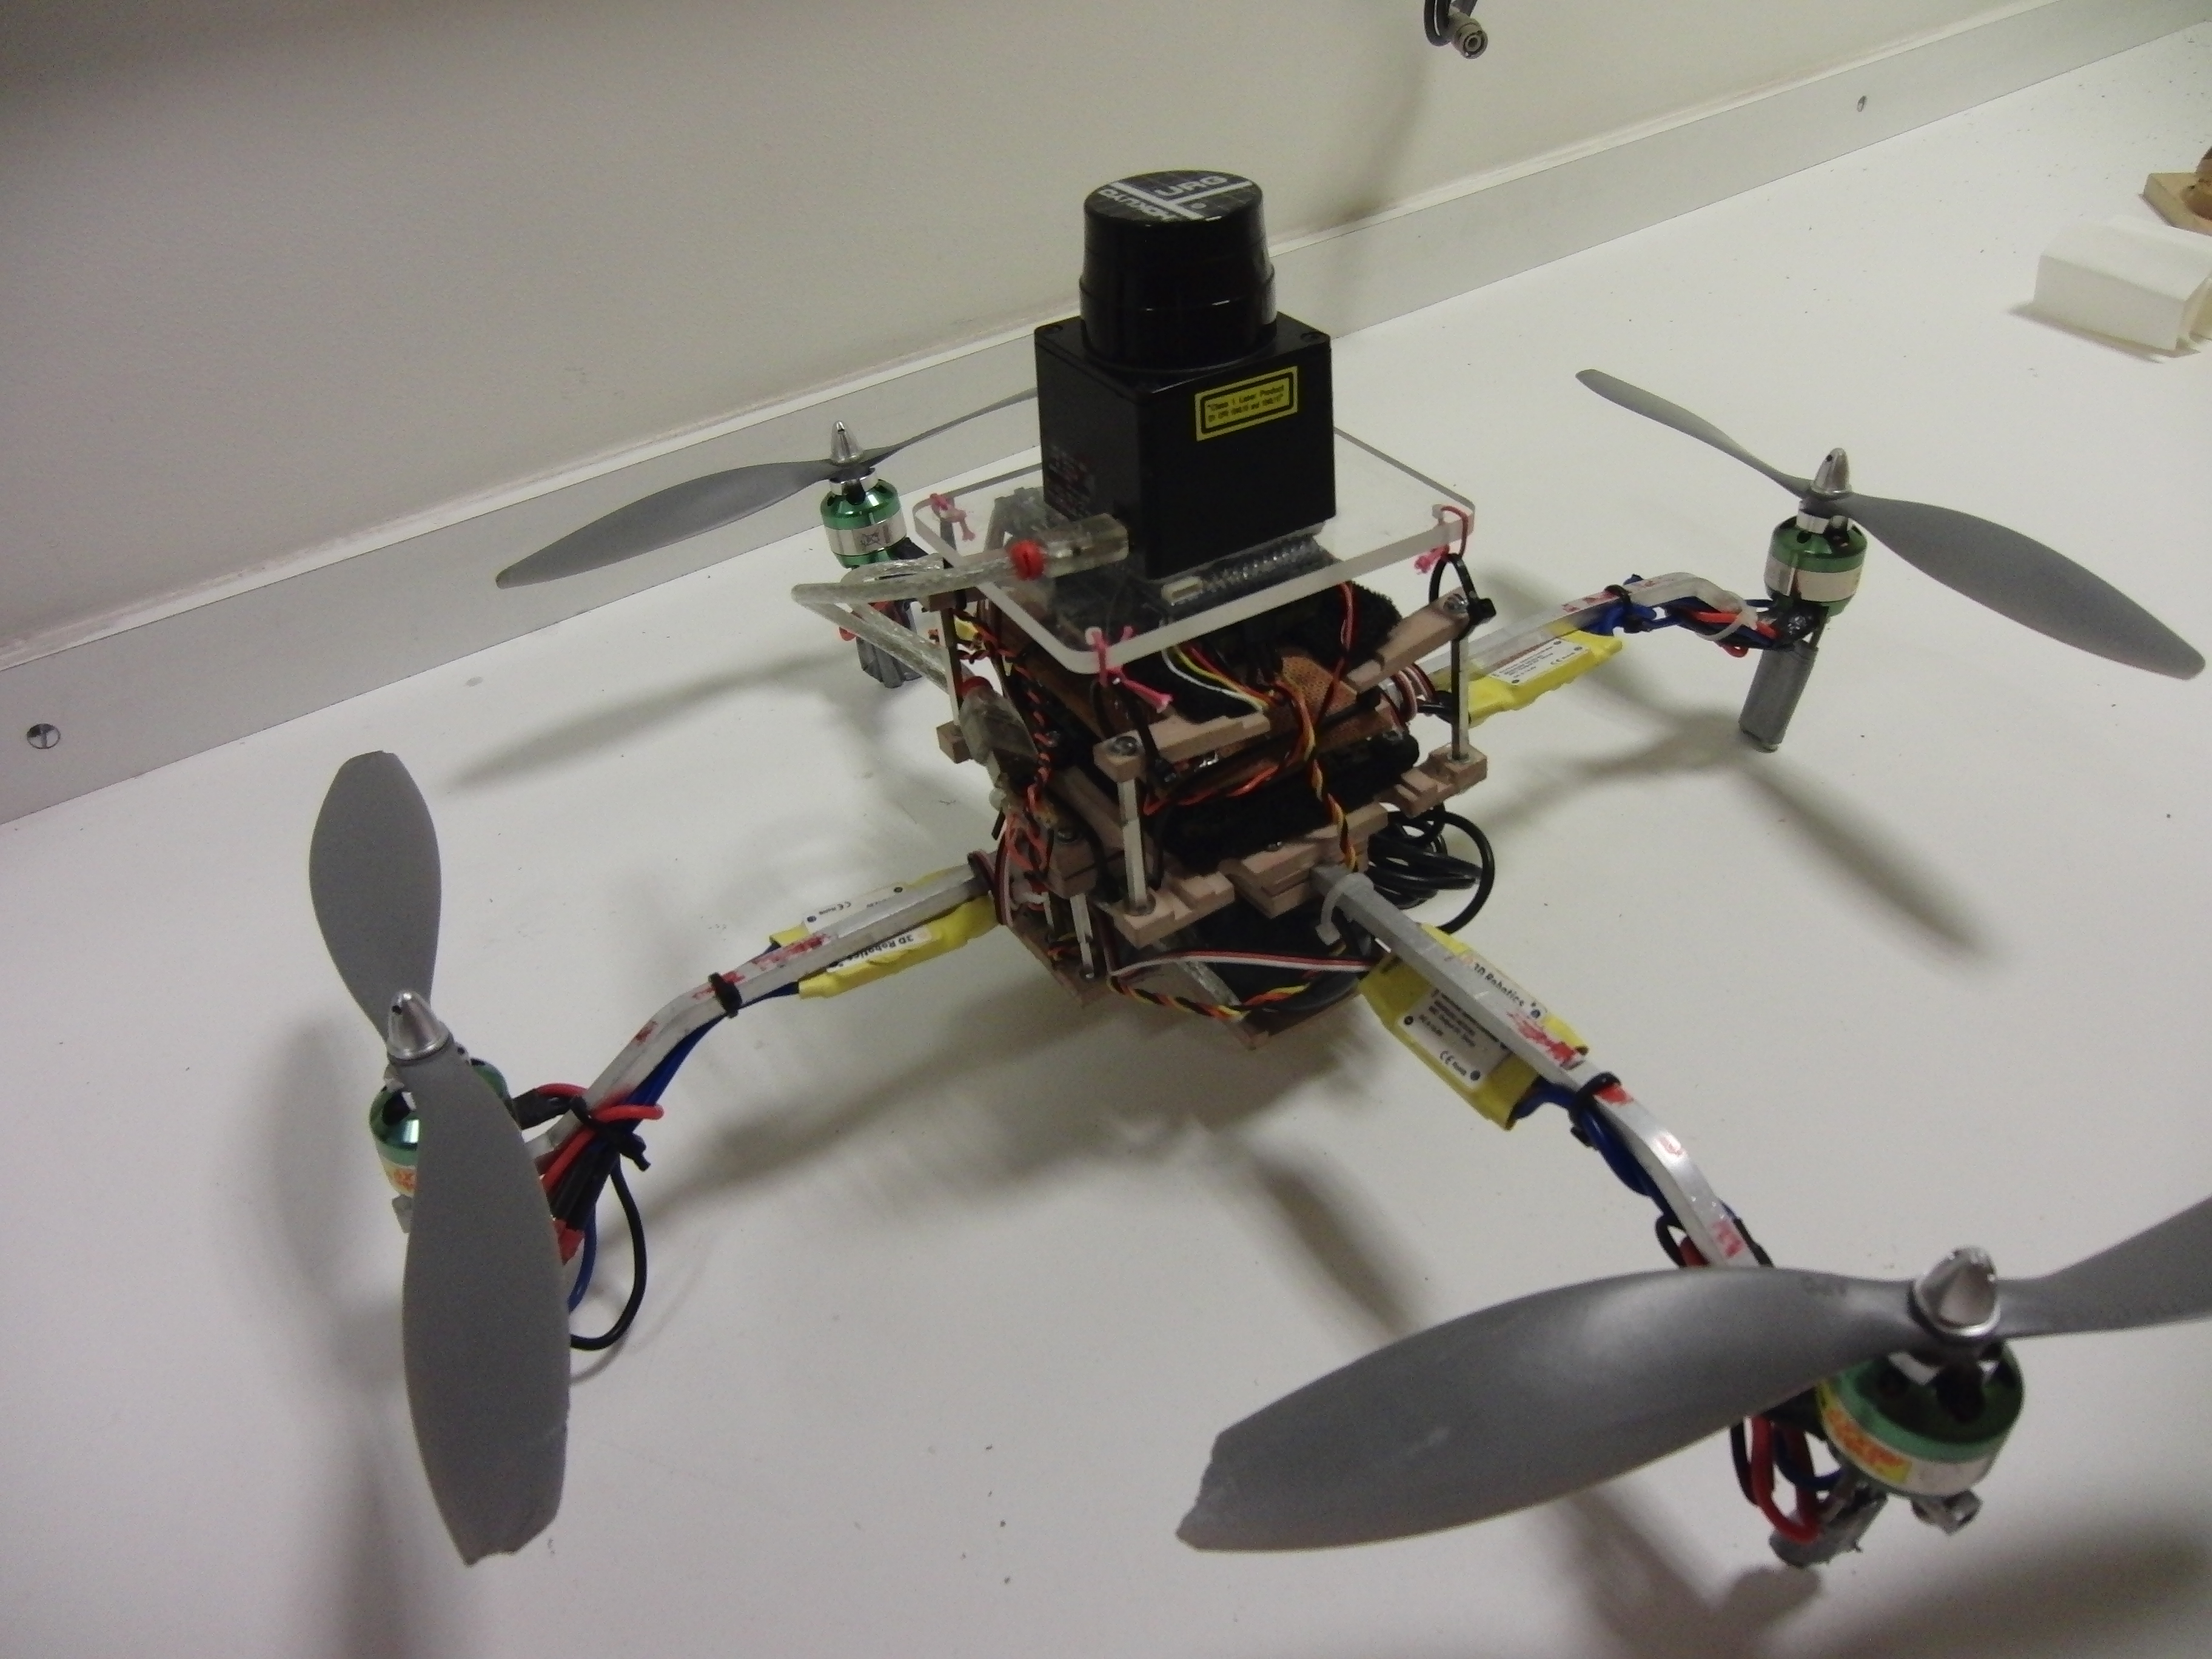
\includegraphics[width=0.65\linewidth]{quadfinal}
	\caption{Het platform wordt in deze figuur weergegeven. De laserscanner is gemonteerd bovenaan de het frame.}\label{fig:quadfinal}
\end{figure}

\subsection{Aanpassingen software}
De nieuwe softwarearchitectuur wordt afgebeeld in figuur \ref{fig:RPIloop3a}. Er verandert echter niets aan de software op de APM, daarom wordt deze niet in detail weergegeven. In de figuur is te zien dat de PC nu twee programma's moet draaien: \textit{SLAM.cpp} en \textit{OpticalFlow.cpp}. Aan de Raspberry Pi kant komt er ook een programma bij: \textit{LaserStream.cpp}.

\begin{figure}[h]
	\centering
	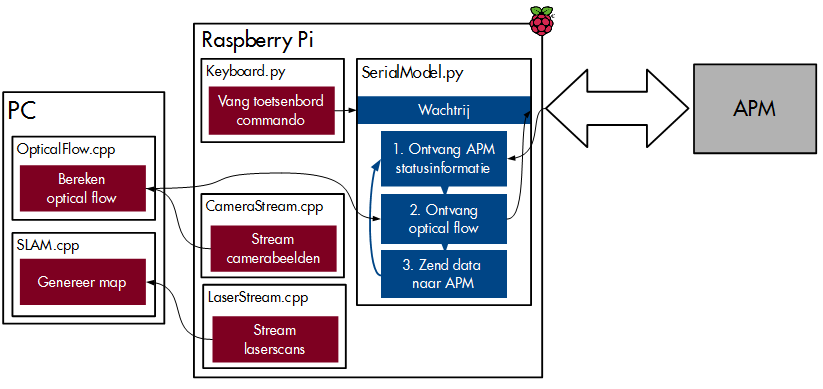
\includegraphics[width=0.8\linewidth]{RPIloop3a}
	\caption{Nieuwe softwarearchitectuur van het platform.}\label{fig:RPIloop3a}
\end{figure}

\subsubsection{LaserStream.cpp}
De naam van dit programma spreekt voor zich. Het is een C programma dat voortdurend scans van de laserscanner doorstuurt naar SLAM.cpp. Voor het versturen wordt een \textit{blocking send} gebruikt. De volgende scan kan pas verstuurd worden wanneer de vorige is ontvangen. Voor het versturen van de scans kunnen de communicatieklassen gebruikt worden die geschreven werden voor de optical flow berekening.

\subsubsection{SLAM.cpp}
SLAM.cpp moet de map genereren met als input de laserscans. Deze worden ontvangen met een \textit{blocking receive}. Het is dan ook niet meer dan logisch dat de volgende schatting van de map pas gemaakt wordt wanneer de nieuwe scan volledig is ontvangen. BreezySLAM voorziet een C bibliotheek met een eenvoudige interface. Deze bibliotheek wordt dan ook gebruikt om het SLAM algoritme te implementeren.

\section{SLAM zonder odometrie}
Eerst wordt het SLAM algoritme ge\"evalueerd zonder het gebruik van odometrie. Het algortime blijkt reeds goed te presteren in een kleine ruimte, zolang \'e\'en bepaalde plaats geen twee maal bezocht wordt. Dit wordt in de literatuur het \textit{loop-closing} probleem genoemd \cite{book:SLAMHandbook}. Als een bepaalde plaats niet herkend wordt wanneer ze voor de twee keer wordt bezocht, dan begint het SLAM algoritme fouten te maken. Een voorbeeld van een kleine map is te zien in figuur \ref{fig:loopclosing}(a). Wanneer een extra rondje gedaan wordt in dezelfde kamer ziet de map eruit als in figuur \ref{fig:loopclosing}(b). Er kan duidelijk gezien worden dat de kamer twee keer boven elkaar wordt getekend. De twee tekeningen van de kamer zijn wat geroteerd ten opzichte van elkaar. Dit doet vermoeden dat het gebruik van odometrie en in het bijzonder, het toevoegen van de yaw van de quadcopter, de gegenereerde map kan verbeteren.

%figuur A kamer 1 rond, B kamer 2 rond
\begin{figure}[h]
	\centering
	\subfigure[Map gegenereerd na \'e\'en rondje in een kamer.]{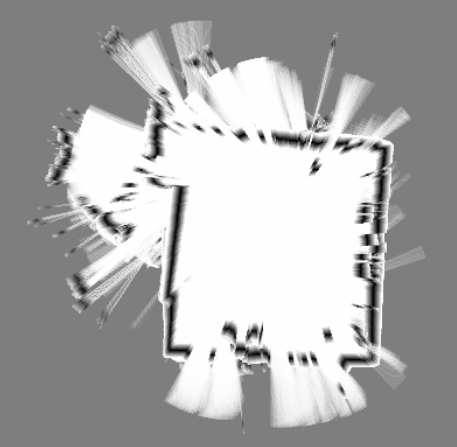
\includegraphics[width=0.40\linewidth, height=6cm]{SLAM/noodo1ROOM}}
	\hspace{0.01\linewidth}
	\subfigure[Map gegenereerd na twee rondjes in een kamer.]{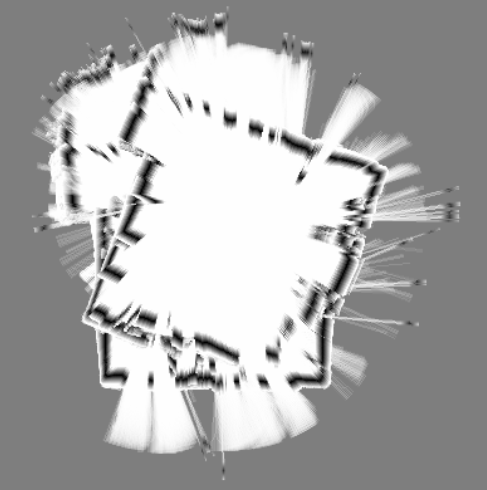
\includegraphics[width=0.40\linewidth, height=6cm]{SLAM/loopclosure}}
	\caption{Het loop-closing probleem: de invloed van eenzelfde plaats twee keer bezoeken. BreezySLAM herkent de plaatsen niet wanneer deze de tweede keer worden bezocht. Hierdoor wordt een nieuwe map getekend bovenop de map die er reeds getekend was.} \label{fig:loopclosing}
\end{figure}

\section{SLAM met odometrie}
Voor het toevoegen van odometrie moeten eerst weer een aantal aanpassingen komen aan de software architectuur. Deze worden eerst beschreven om vervolgens over te gaan tot de resultaten. De finale versie van de architectuur is afgebeeld in figuur \ref{fig:RPIloop3}.

\begin{figure}[h]
	\centering
	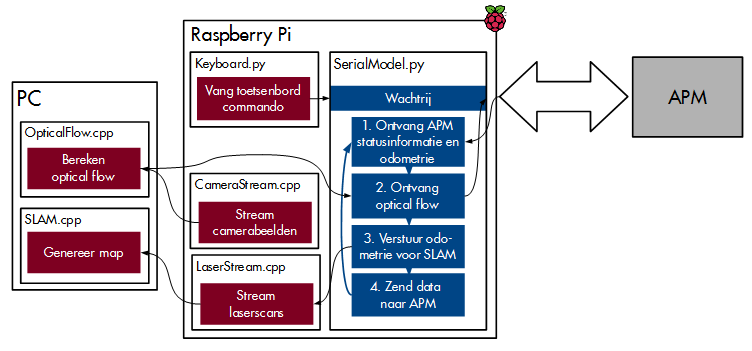
\includegraphics[width=0.8\linewidth]{RPIloop3}
	\caption{De aangepaste architectuur, die SLAM voorziet van odometrie.} \label{fig:RPIloop3}
\end{figure}

\subsection{Aanpassingen softwarearchitectuur}
De odometrie moet vanop de APM tot aan SLAM.cpp op de PC geraken. BreezySLAM vraagt de voorwaartse verplaatsing, het verschil in yaw en het tijdsverschil waarover deze twee werden gemeten als odometrie. Het aanpassen van de APM is triviaal gezien dit gewoon betekent dat specifieke statusinformatie geprint moet worden naar de RPi. Binnen SLAM.cpp moet de odometrie gewoon als extra parameter meegegeven worden aan BreezySLAM. De andere aanpassingen zijn iets minder triviaal en worden daarom wat uitgebreider beschreven. Het compenseren van de laserscans met roll en pitch van het platform wordt voorlopig nog niet ge\"implementeerd omdat er verondersteld wordt dat de quadcopter gedurende zijn vlucht altijd ongeveer evenwijdig met de grond blijft vliegen.

\subsubsection{SerialModel.py}
In het serieel model, \textit{SerialModel.py}, van de RPi moet de statusinformatie met odometrie doorgewezen worden naar het programma LaserStream.cpp. De software van de RPi zal er uit zien zoals op figuur \ref{fig:RPIloop3}. Er is een taak bijgekomen in de lus. Telkens wanneer odometrie beschikbaar is wordt die met een \textit{blocking send} doorgestuurd naar het programma LaserStream.cpp.

\subsubsection{LaserStream.cpp}
In LaserStream.cpp wordt een aparte thread aangemaakt die voortdurend wacht tot er nieuwe odometrie beschikbaar is. Om de odometrie te ontvangen wordt een \textit{blocking receive} gebruikt. Odometrie wordt ge\"updatet aan de snelheid waarmee een nieuwe voorwaartse verplaatsing beschikbaar is. Uit tabel \ref{table:resolutieRPI} bleek dat dit voor de RPi2 aan \SI{30}{\Hz} is. Om het verschil in snelheid tussen de odometrie en de laserscan op te vangen, wordt de odometrie geaggregeerd zolang er geen scan beschikbaar is. Wanneer een nieuwe scan klaar is om te verzenden wordt de geaggregeerde odometrie eraan toegevoegd. Om ervoor te zorgen dat dit alles \textit{thread-safe} gebeurt, wordt gebruik gemaakt van een \textit{mutex}.

\subsection{Resultaat}
Om het resultaat van de toevoeging van de odometrie te kunnen evalueren wordt telkens vergeleken met de resultaten zonder odometrie. In figuur \ref{fig:BreezyRes}(a) en \ref{fig:BreezyRes}(b) wordt een map weergegeven van \'e\'en kamer respectievelijk zonder en met odometrie. In figuur \ref{fig:BreezyRes}(c) en \ref{fig:BreezyRes}(d) wordt een map weergegeven van drie kamers respectievelijk zonder en met odometrie.

\npar Voor het mappen van \'e\'en kamer is de prestatie met en zonder odometrie ongeveer dezelfde. Wanneer meerdere kamers in kaart worden gebracht, draaien ze wat ten opzichte van elkaar als geen odometrie wordt gebruikt. Wanneer wel rekening gehouden wordt met odometrie, liggen de kamers correcter naast elkaar.

\npar In figuur \ref{fig:loopclosing2} wordt het loop-closing probleem zonder en met odometrie vergeleken. Ook met odometrie heeft BreezySLAM het moeilijk om een goede map te genereren wanneer een bepaalde plaats meer dan eens wordt bezocht. Het ontbreken van een loop-closing strategie blijft een pijnpunt. Het huidige algoritme moet dus uitgebreid worden om betere mappen te kunnen genereren. Overstappen naar een ander algoritme, dat wel aan loop-closing doet is ook een optie.

\npar Om te zien of het op termijn mogelijk zou zijn om de RPi\,2 te gebruiken voor omgevingsmapping zonder hulp van de PC, wordt al eens gekeken naar het CPU gebruik bij het uitvoeren van BreezySLAM. Dit blijkt 37\% te bedragen. Een zwaarder algoritme draaien is dus nog mogelijk.

\section{Besluit}
Het toevoegen van odometrie aan BreezySLAM zorgt reeds voor betere mappen. Toch zijn ze nog niet nauwkeurig genoeg. De reden voor deze ondermaatse prestatie ligt bij het ontbreken van een loop-closing stategie. TinySLAM doet wel aan loop-closing en is dus een optie. HectorSLAM doet niet aan loop-closing, maar uit onderzoek blijkt dat het algoritme toch nauwkeurig genoeg werkt zonder \cite{paper:hectorSLAM}.

\npar Het platform slaagt er nu nog niet in om consequent goede mappen te genereren. Er is echter wel nog ruimte voor verbetering, gezien het processor maar voor 37\% belast wordt wanneer de map gegenereerd wordt door de RPi zelf. Er is niet alleen ruimte voor verbetering, er is ook nog ruimte om programma's te draaien die instaan voor autonome exploratie en het ontwijken van obstakels.

\begin{figure}
	\centering
	\subfigure[Map van 1 kamer, gegenereerd zonder odometrie]{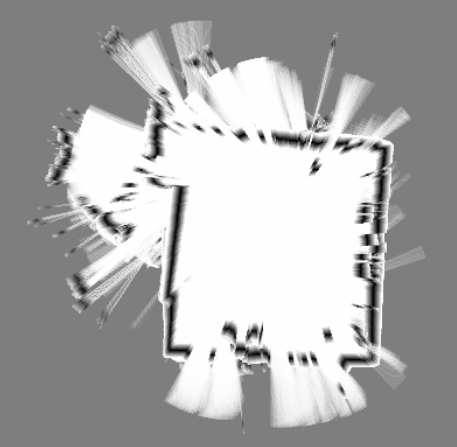
\includegraphics[width=0.45\linewidth, height=7cm]{SLAM/noodo1ROOM}}	
	\hspace{0.01\linewidth}
	\subfigure[Map van 1 kamer, gegenereerd met odometrie]{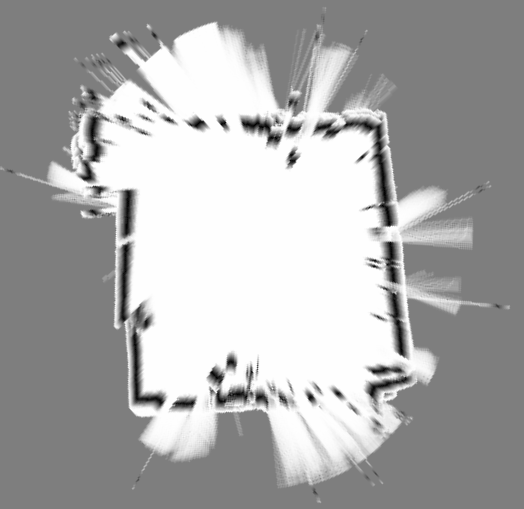
\includegraphics[width=0.45\linewidth, height=7cm]{SLAM/odo1ROOM}}
	
	\subfigure[Map van 3 kamers, gegenereerd zonder odometrie]{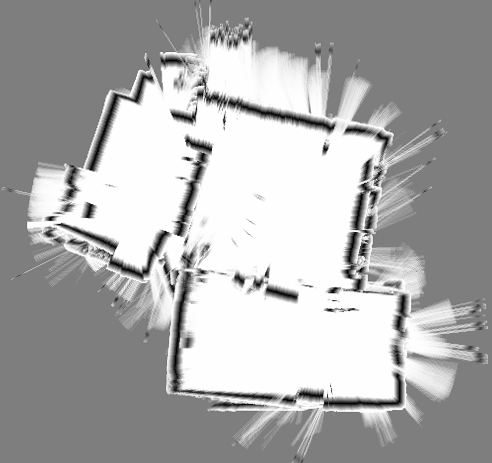
\includegraphics[width=0.45\linewidth, height=6cm]{SLAM/noodo3ROOMS}}
	\hspace{0.01\linewidth}
	\subfigure[Map van 3 kamers, gegenereerd met odometrie]{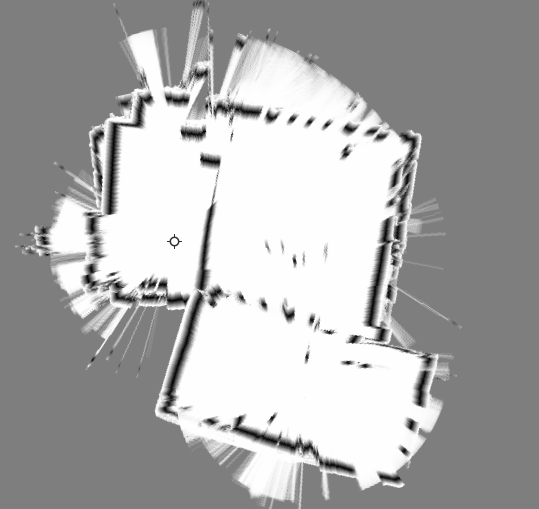
\includegraphics[width=0.45\linewidth, height=6cm]{SLAM/odo3ROOMS}}
	\caption{Vergelijking tussen de prestatie van BreezySLAM met en zonder odometrie. Om deze mappen te genereren werd het meermaals bezoeken van eenzelfde plaats vermeden. De prestatie van BreezySLAM met en zonder odometrie is ongeveer dezelfde wanneer een kleine ruimte gemapt wordt. Als drie aaneensluitende ruimtes gemapt moeten worden roteren ze wat ten opzichte van elkaar wanneer geen odometrie wordt gebruikt. Als wel odometrie wordt gebruikt, liggen de kamers correcter ten opzichte van elkaar.}\label{fig:BreezyRes}
\end{figure}

\begin{figure}
	\centering
	\subfigure[Loop-closing zonder odometrie]{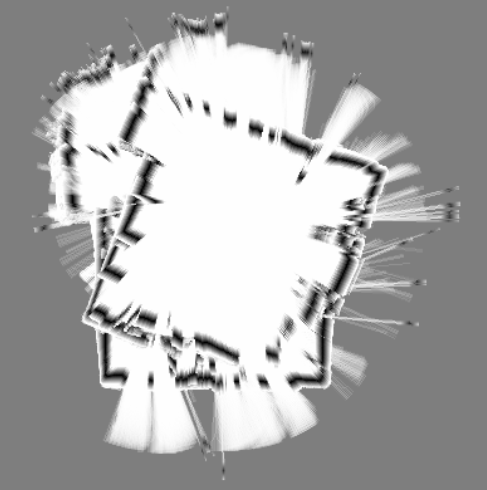
\includegraphics[width=0.45\linewidth, height=7cm]{SLAM/loopclosure}}	
	\hspace{0.01\linewidth}
	\subfigure[Loop-closing met odometrie]{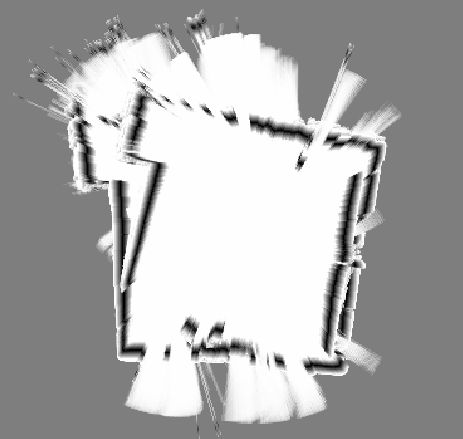
\includegraphics[width=0.45\linewidth, height=7cm]{SLAM/odoloopclosing}}
	\caption{Loop-closing vergeleken voor BreezySLAM zonder(a) en met(b) odometrie. Het meermaals bezoeken van eenzelfde plaats blijft een probleem, ook wanneer odometrie gebruikt wordt.} \label{fig:loopclosing2}
\end{figure}

